\documentclass[a4paper,11pt,oneside]{mybook}
\usepackage{latexsym}
\usepackage{amsmath}
\usepackage{amsfonts}
\usepackage{amsthm}
\usepackage{amssymb}
\usepackage{fncylab}

%fonty
\usepackage{charter}
\usepackage{euler}

% tiskove zrcadlo
\topmargin-40pt
\headheight15pt
\headsep10pt
\topskip0pt
\textheight700pt
\oddsidemargin-20pt
\evensidemargin-20pt
\textwidth500pt

\usepackage{graphicx}

%headings
\usepackage{fancyhdr}
\pagestyle{myheadings}
\pagestyle{fancy}

%----------definitions---------------------------
\def\R{\mathbb R}
\def\cl{\text{cl}}
\def\norma#1{\parallel\!#1\!\parallel}
\def\norm#1{\parallel\!#1\!\parallel}

%math definitions
\def\sub{\text{Sub}}
\def\meas{\text{Meas}}
\def\msub{\text{mSub}}
\def\cov{\text{cov}}
\def\cal{\text{cal}}
\def\msubn{\text{mSub}_{\text{1}}}
\def\subn{\text{Sub}_{\text{1}}}
\def\fn{\text{Fn}}

\def\B{{\mathbb B}}
\def\C{{\mathbb C}}

\def\F{{{\mathcal F}}}
\def\N{{{\mathcal N}}}

\def\cont{{2^{\aleph_0}}}
\def\force{\Vdash}
\def\aleq{\leq^{*}}
\def\succ{\hbox{succ}}
\def\pw{{{\mathcal P}}}
\def\conc{{^\smallfrown}}

\def\dom{\hbox{dom}}
\def\pomega{\pw(\omega)}
\def\0{\hbox{\bf 0}}
\def\1{\hbox{\bf 1}}
\def\intr#1{%
  \hbox{int}\ #1%
}
\def\cl#1{%
  \hbox{cl}\ #1%
}



%---------numbering of the formulas and theorems---------------
% \newcounter{thm}[section]
% \numberwithin{thm}{section}

%---------numbering of the theorems------------
\swapnumbers

%\theoremstyle{plain}
\newtheoremstyle{theorem}% name
  {}%      Space above
  {}%      Space below
  {\itshape}%         Body font
  {}%         Indent amount (empty = no indent, \parindent = para indent)
  {\bfseries\scshape}% Thm head font
  {.}%        Punctuation after thm head
  {.5em}%     Space after thm head: " " = normal interword space;
        %       \newline = linebreak
  {}%         Thm head spec (can be left empty, meaning `normal')
\theoremstyle{theorem}
\newtheorem*{theorem*}{Theorem}
\newtheorem{theorem}[subsection]{Theorem}
\newtheorem{lemma}[subsection]{Lemma}
\newtheorem{proposition}[subsection]{Proposition}
\newtheorem{fact}[subsection]{Fact}
\newtheorem{claim}[subsection]{Claim}
\newtheorem{corollary}[subsection]{Corollary}
\newtheorem{problem}[subsection]{Problem}
%\numberwithin{equation}{section}
%\theoremstyle{definition}
\newtheorem{definition}[subsection]{Definition}
\newtheorem{notation}[subsection]{Notation}
%\theoremstyle{remark}
\newtheorem{remark}[subsection]{Remark}
\newtheorem*{note}{Note}
\newtheoremstyle{example}% name
  {}%      Space above
  {}%      Space below
  {}%         Body font
  {}%         Indent amount (empty = no indent, \parindent = para indent)
  {\bfseries\scshape}% Thm head font
  {.}%        Punctuation after thm head
  {.5em}%     Space after thm head: " " = normal interword space;
        %       \newline = linebreak
  {}%         Thm head spec (can be left empty, meaning `normal')
\theoremstyle{example}
\newtheorem{example}[subsection]{Example}

%\labelformat{subsection}{\thechapter.#1}

%vytvoreni indexu
\usepackage{makeidx}
\makeindex


\pdfinfo{
     /Author (Jonathan Verner)
     /Title (Laver forcing)
     /Subject (forcing, set theory)
     /Keywords (laver forcing, trees)
  }

\bibliographystyle{mujstyl}
%-------------opening--------------------------
\begin{document}
\cfoot{}\rhead{\thepage}
\lhead{{\scshape Laver forcing} $\qquad$ {\tiny \today } }

\noindent{\Large{\scshape\bfseries Entr\'e to Generic Extensions and Forcing in Set Theory}} \\[0.1cm]

\noindent {\scshape Bohuslav Balcar}, {\small CTS, J{\' \i}lsk{\' a} 1, Praha 1,
	Czech Republic, {\ttfamily balcar@cts.cuni.cz} } \\[0.1cm]
\noindent {\scshape Tom\'a\v{s} Paz\'ak}, {\small CTS, J{\' \i}lsk{\' a} 1, Praha 1,
	Czech Republic, {\ttfamily balcar@cts.cuni.cz} } \\[0.1cm]
\noindent {\scshape Jonathan Verner}, {\small KTIML MFF UK,
	Czech Republic, {\ttfamily jonathan.verner@matfyz.cz} }\\[0.1cm]
{\tiny \today } \\[0.5cm]

%\maketitle

\thispagestyle{empty}

\section{Laver forcing}

In this section we show the basic properties of Laver forcing. Recall the that the laver forcing $\mathbb{L}$ consists of $\omega$-ary $\omega$-branching
trees with a stem, i.e.
$$
\mathbb{L}=\{T\subseteq {}^{<\omega}\omega:(\forall \sigma\in T)(stem(T)\subseteq \sigma\rightarrow |succ_{T}(\sigma)|=\omega\}.
$$

For $\sigma\in T$ we have defined $T_\sigma=\{\tau\in T:\sigma\subseteq \tau\}$. Also recall that given a tree $T\subseteq{}^{<\omega}\omega$, the set of leafs is
$$
Lf(T)=\{\tau\in T:(\forall\sigma\in{}^{<\omega}\omega)(\tau\subseteq\sigma\ \&\ \sigma\in T\rightarrow \sigma=\tau)\}.
$$
For a condition $p\in \mathbb{L}$ a $\sigma\in p$ and a name $\dot{f}$ for a function from $\omega$ to $\omega$ we shall write
$$
\dot{f}[\sigma,p]=\bigcup\{g\in{}^{<\omega}\omega:p_\sigma\force g\subseteq f\},
$$
in other words $\dot{f}[\sigma,p]$ is the largest segment of $\dot{f}$ decided by $p_\sigma$. When $p$ is clear from the context, we omit it.

Recall, that the method of \emph{fusion} is a standard tool for laver forcing. Suppose $T\in\mathbb{L}$ and assume that for each $\sigma\in T$,
the set $succ_T(\sigma)$ is enumerated in increasing order as $\{a_\sigma^i:i<\omega\}$. Define for $n<\omega$ the following
$$
B(T,n)=\{\sigma\in T:(\forall i <\omega)(\sigma(i)\leq a_(\sigma\upharpoonright i)^i)\ \&\ |\sigma|\leq|stem(T)|+n\}.
$$
For $T,S\in\mathbb{L}$ we say that $T\leq_n S$ if $B(T,n)=B(S,n)$. If $T,S$ are identical up to the $n$-th splitting level we say that
$T\leq_n S$. It is clear that $T\preceq_n S\rightarrow T\leq_n S$. The `fusion method' lies in the observation that given a sequence $\langle T_n:n<\omega\rangle$
of laver conditions such that $T_{n+1}\leq_n T_n$ then $\bigcap_{n<\omega} T_n$ is again a laver condition.

The following fact is easy

\begin{fact} Laver forcing adds a dominating real, i.e. there is a name $\dot{r}$ such that for any $f\in{}^{<\omega}\omega$ and $p\in\mathbb{L}$
there is a $q\in\mathbb{L}$ such that $q\leq p$ and $q\force \check{f}\leq^* \dot{r}$.
\end{fact}

We shall show that Laver adds a dominating family of size $\omega_1$ so $\mathbb{L}\force\mathfrak{d}=\check{\omega}_1$. Notice that this implies that
Laver forcing does not collapse $\omega_1$, since a dominating family cannot be countable.


\begin{theorem}\label{dominating-family} Laver forcing adds a dominating family of size $\omega_1$.
\end{theorem}

Before we prove the theorem, we shall show that Laver satisfies the so called ''strong fusion'':

\begin{proposition} For any $S\in\mathbb{L}$ and $D_n$ ($n<\omega$) a countable family of open dense sets
there is stronger condition $T\leq S$ such that for each $n<\omega$ the set
$$\{\sigma\in T:T_\sigma\in D_n\}$$
intersects every branch of $T$, i.e. $(\forall f\in [T])(\exists m<\omega)(T_{f\upharpoonright m}\in D_n)$.
\end{proposition}
\begin{proof} (due to Judah and Shelah, \cite{judah-shelah}) We shall build a fusion sequence $T^n$ such that $T^{n+1}$ satisfies the requirement for $D_n$. It is easy
to see that the fusion tree $T=\bigcap_{n<\omega}T^n$ will be as required. We start by letting $T^0=S$ and proceed by
induction. Suppose then, that we have constructed $T^n$ and let $Lf_n(T^n)$ be the $n$-th level of $T^n$ above the stem,
i.e.
$$Lf_n(T^n) = \{\sigma\in T^n:|dom(\sigma)|-|dom(stem(T^n))|=n\}.$$

For each $\tau\in Lf_n(T^n)$ we find a suitable tree $T(\tau)\leq T^n_\sigma$ and then let $T^{n+1}=\bigcup \{T(\tau):\tau\in Lf_n(T^n)$.
This will clearly give us $T^{n+1}\leq_n T^n$ (even $T^{n+1}\preceq_n T^n$, so we only need to guarantee the requirement for $D_n$. Given $\tau\in Lf_n(T^n)$ we
label the nodes $\sigma\in T^n_\tau$ extending $\tau$ with ordinals by recursion as follows:
$$
\rho(\sigma)=0\iff(\exists S\leq_0 T^n_\tau)(S\in D_{n+1})
$$
and
$$
\rho(\sigma)=\min\{\alpha:(\exists^{\infty} n)(\sigma\conc n\in T^n_\tau\ \&\ \rho(\sigma\conc n)<\alpha)\}.
$$
If $\rho(\sigma)$ is undefined, we let $\rho(\sigma)=\infty$.

\begin{claim} $\rho(stem(T^n_\tau))<\omega$
\end{claim}
If $\rho(\sigma)=\infty$ then there is a $k_\sigma<\omega$ such that for all $n\geq k_\sigma$ if $\sigma\conc n\in T^n_\tau$ then $\rho(\sigma\conc n)=\infty$.
So if $\rho(\sigma)=\infty$ we can build a laver condition $S\leq_0 T^n_\tau$ such that $\rho[S]=\{\infty\}$. Since $D_{n+1}$ is open dense,
there must be a $S^\prime\leq S$ such that $S\in D_{n+1}$. Let $\sigma=stem(S^\prime)$. Then, by definition, $\rho(\sigma)=0$ which is a contradiction.

It is now easy to prune the tree $T^n_\tau$ into a laver tree $T(\tau)$  so that $\rho$ is strictly decreasing (until it attains the value $0$) along the branches of $T(\tau)$ and so that if $\sigma\in T(\tau)$ is labeled with $0$, then $T(\tau)_\sigma\in D_{n+1}$.

Clearly the tree
$$T^{n+1}=\bigcup_{\tau\in Lf_n(T^n)} T(\tau)$$
will satisfy the requirement.
\end{proof}

\begin{proof}[Proof of theorem \ref{dominating-family}] Since Laver adds a dominating real, we need not worry about ground-model reals. The hard part is to ensure that the dominating family dominates all new reals. The proof is due to J. Brendle (see \cite{brendle-combinatorial}).

We will try to motivate the proof which is somewhat formally compicated. It is instructive to think of a name $\dot{f}$ as a program, which, given a generic on the input,
outputs the evaluation $\dot{f}[G]$. In the case of a Laver forcing, the generic can be thought of as a sequence of natural numbers --- the Laver real. Consider a name
$\dot{f}$ for a function from $\omega$ to $\omega$ and think of it as a program. Now suppose we want to know the value $\dot{f}[G](n)$. It may happen, that we only need a finite amount of information about $G$ to know this value. For example, if $\dot{f}(n)=G(n)+1$, then to determine the first $n$ values of $\dot{f}[G]$ we only need to
know the first $n$ values of $G$. Or if $\dot{f}(n)=G(2n)+G(2n+1)$, we will need the first $2n$ values.

Now suppose we have two names $\dot{f}$,$\dot{g}$ for reals and a condition $p\in\mathbb{L}$. Furthermore imagine that the programs (names) $\dot{f}$,$\dot{g}$ have the following property: For each $n$ the program $\dot{f}$ always outputs the $n$-th value strictly earlier than the program $\dot{g}$ when they are given an input sequence which is a branch of $p$. Furthermore assume that the program $\dot{g}$ can only output the value of the input it is currently reading (i.e. either it outputs nothing and reads another member of the input sequence, or it outputs the value just read). We can then conclude that $p\force \dot{f}(n)\leq^*\dot{g}(n)$. To see this, note that given a $q\leq p$, and $m>|stem(q)|$ go along a branch of $q$ until $\dot{f}$ outputs the $m$-th value, say $k$. At this point $\dot{g}$ did not yet output the $m$-th value. Suppose that we have went along $\sigma\in q$. We can now prune $q$ by discarding all branches not extending $\sigma$ or having values $\leq k$ after $\sigma$. This gives us a condition $q^\prime\leq q$ and necessarily $q^\prime\force k=\dot{f}(m)\leq\dot{g}(m)$, since $\dot{g}$ cannot output anything smaller than $k$ when given an input sequence which is a branch of $q^\prime$.

The idea of the proof is to find a sequence of names $\dot{g}_\alpha$ ($\alpha<\omega_1$) such that for each name $\dot{f}$ there is an $\alpha<\omega_1$ such that $\dot{f}$ and $\dot{g}$ satisfy the assumptions of the preceding paragraph. We shall now try to formalize this.


First, given a condition $p\in\mathbb{L}$ a name $\dot{f}$ for a real number, $\sigma\in p$ and $n<\omega$. Starting at $\sigma$ we want to estimate how far along a branch of $p$ we must go, in order to know the value of $\dot{f}(n)$. We first build a tree $T^{\dot{f}}(n)\subseteq p_\sigma$ by going along branches of $p_\sigma$ and putting the nodes encountered into $T^{\dot{f}}(n)$ until some node decides the value of $\dot{f}(n)$. Then we stop. We shall show, that this process will make $T^{\dot{f}}(n)$ an illfounded tree and the rank of this tree will be our estimate of the distance. Formally let
$$D_n=\{q\in\mathbb{L}:q\parallel \dot{f}\upharpoonright n\}.$$
Each $D_n$ is an open dense subset of $\mathbb{L}$. Use strong fusion to find a stronger condition $q\leq p$ such that
$$
\{\sigma\in q:q_\sigma\in D_n\}
$$
intersects every branch of $q$. Now define the trees
$$
T^{\dot{f}}(n)=\{\sigma\in q:(\forall\tau\subsetneq\sigma)(q_\sigma\not\in D_n)\}.
$$
Strong fusion guarantees that $T^{\dot{f}}(n)$ is an illfounded tree. Given a $\sigma\in q$ we define the ``distance to $n$'', $d^{\dot{f}}(\sigma,n)$, to be the rank of the tree $T^{\dot{f}}(n)_\sigma$, tacitly assuming that the rank of $T^{\dot{f}}(n)_\sigma$ is $0$ when $\sigma\not\in T^{\dot{f}}(n)$.

Now we define the names of the dominating functions $\{\dot{g}_\alpha:\alpha<\omega_1\}$. We will define them in such a way, that if $\sigma\in p$ is the first
$\sigma$ which decides $\dot{g}_\alpha(n)$ then $d^{\dot{g}_\alpha}(\sigma,n+1)\geq\alpha$.

We need some preparation first. Recall that for every $\alpha<\omega_1$ there is a tree $T_\alpha$ of rank $\alpha$. By induction on $n<\omega$ we define for each $\alpha<\omega$ the trees $T_\alpha^n$. We let $T_\alpha^0=T_\alpha$ and then carry on by gluing $T_\alpha^0$ to the leafs of $T_\alpha^n$ to obtain $T_\alpha^{n+1}$, formally:
$$
T_\alpha^{n+1}=\{\sigma:\sigma=\tau\conc\nu,\quad\mbox{where}\ \tau\in Lf(T_\alpha^n)\ \&\ \nu\in T_\alpha\}\cup T_\alpha^n.
$$
Also define
$$
L_\alpha^n=Lf(T_\alpha^n).
$$
Notice that for each $\alpha<\omega$ the $T_\alpha^n$'s cover ${}^{<\omega}\omega$, i.e. $\bigcup_{n<\omega}T_\alpha^n={}^{<\omega}\omega$.
Given $\sigma\in{}^{<\omega}\omega$, we let $k_\alpha(\sigma)=\min\{k:\sigma\in T_\alpha^k\}$, i.e. the first $k$ such that $\sigma$ is covered by $T_\alpha^k$, and for $n<k_\alpha(\sigma)$ we let $l_\alpha^\sigma(n)$=$|\sigma\cap L_\alpha^n|$, that is $l_\alpha^\sigma(n)$ is the length of the smallest initial segment of $\sigma$ which falls in $L_\alpha^n$. Now we can define the projection $\pi_\alpha^\sigma\in{}^{<\omega}\omega$ of $\sigma$ as follows:
$$
\pi_\alpha^\sigma(n)=\sigma(l_\alpha^\sigma(n)),\quad n<k_\alpha(\sigma)
$$
In other words to determine the value of $\pi_\alpha^\sigma$ at $n$, go along $\sigma$ until you are at the first node in $L_\alpha^n$. The required value
is the value of this node (see picture).
\vskip5mm
\centerline{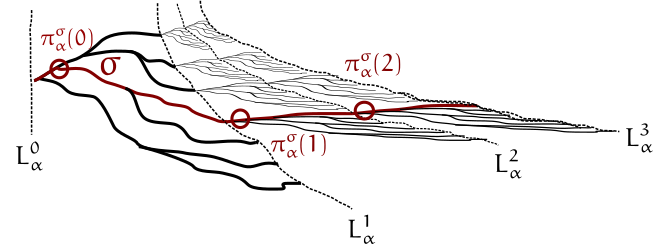
\includegraphics[scale=0.40]{laver-picture.pdf}}

Now we are ready to define the names $\dot{g}_\alpha$. Fix a name $\dot{r}$ for the generic dominating real. Given a condition $p\in\mathbb{L}$ let $\sigma_p\in{}^{<\omega}\omega$ be maximal such that $p\force\sigma_p\subseteq\dot{r}$.
Now define names $\dot{g}_\alpha$ such that given $p\in\mathbb{L}$, $p$ decides at most $k_\alpha(\sigma_p)$ values of $\dot{g}_\alpha$ and
$$
p\force \dot{g}_\alpha\supseteq \pi_\alpha^{\sigma_p}.
$$

\begin{claim} $\{\dot{g}_\alpha:\alpha<\omega_1\}$ is a dominating family.
\end{claim}

Given a name $\dot{f}$ for a function from $\omega$ to $\omega$ let $\bar{\alpha}=\sup\{d^{\dot{f}}[p\times\omega]\}$, i.e. $\bar{\alpha}$ is bigger
than any ``distance'' from $\sigma$ to $n$ in $p$. We shall show that for each $\alpha$ there is a stronger condition $q\leq p$ such that
$$
q\force \dot{f}\leq^*{\dot{g}_\alpha}.
$$

Let ``$k=|stem(p)|$''. We build the condition $q$ by recursion on the levels of $p$ putting in $q$ some nodes of $p$ so that the following is satisfied for $\tau\in q$ and
$k<n<\omega$
\begin{itemize}
 \item[(i)] Either $0=d^{\dot{f}}(\tau,n)=d^{{\dot{g}_\alpha}}(\tau,n)$ and $\pi_\alpha^\tau(n)>\dot{f}[\tau](n)$ or
 \item[(ii)] $0\leq d^{\dot{f}}(\tau,n)<d^{{\dot{g}_\alpha}}(\tau,n)$.
\end{itemize}
It is clear, that if we can guarantee that $q\in \mathbb{L}$, then $q\leq p$ and (i) witnesses $q\force\dot{f}\leq^*{\dot{g}_\alpha}$. Condition (ii) is used to keep the
recursion going.

We prove that $q$ can be built into a laver condition. Assume we have put $\tau$ in $q$. Let $m$ be minimal such that $d^{{\dot{g}_\alpha}}(\tau,m) > 0$. There are two
cases.

{\bf Case 1.} $0=d^{\dot{f}}(\tau,m) < d^{{\dot{g}_\alpha}}(\tau,m)=1$. We put $\tau\conc i$ into $q$ for all $i > \dot{f}[\tau](n)$ such that $\tau\conc i\in p$.

{\bf Case 2.} $\beta=d^{\dot{f}}(\tau,m) < d^{{\dot{g}_\alpha}}(\tau,m)=\gamma$. If $\gamma$ is a successor, then we can put all $\tau\conc i$ into $q$ for all $i$ such that
$\tau\conc i\in p$, since $d^{{\dot{g}_\alpha}}(\tau\conc i,m)=\gamma-1>d^{\dot{f}}(\tau\conc i,m)$. In case $\gamma$ is limit, the equation
$$
d^{{\dot{g}_\alpha}}(\tau\conc i,m)=\gamma-1>d^{\dot{f}}(\tau\conc i,m)
$$
is true for almost all $i$, so we can put $\tau\conc i$ into $q$ whenever $\tau\conc i\in p$ and $i$ satisfies the equation.

Since in each step we have added an infinite (even cofinite) number of successors to a given $\tau\in q$ we conclude that $q$ is indeed a laver tree and
this finishes the whole proof.

\end{proof}


\begin{definition} A forcing $P$ has the \emph{laver property} if each bounded function from the extension can be covered by a tunnel of bounded diameter. Formally
if $\dot{f}$ is a name for a function from $\omega$ to $\omega$ and there is some $g$ and $p\in P$ such that $p\force \dot{f}\leq g$, then there is a tunnel
$F:\omega\to[\omega]^{<\omega}$ together with a condition $q\leq p$ such that $q\force(\forall n<\omega)(\dot{f}(n)\in F(n))$ and $|F(n)|\leq n^n$.
\end{definition}

\begin{theorem} Laver forcing has the laver property.
\end{theorem}
\begin{proof} Following \cite{bartoszynski-judah} we prove that $\mathbb{L}$ has a stronger property, namely that it satisfies $L_f$ for $f=n^n$.

Given $f\in{}^\omega\omega$ we say that $\mathbb{L}$ satisfies property $L_f$ if for any name $\dot{a}$ and a condition $T\in\mathbb{L}$ such
that $T\force\dot{a}\in A$ for some finite $A$, there is for each $n$ a stronger condition $T^\prime\leq_n T$ and $B$ of size $\leq f(n)$ such that $T^\prime\force \dot{a}\in B$.

It is easy to see that $L_f$ for $f=n^n$ implies the laver property: Given a name $\dot{f}$ and a condition $p$ use $L_f$ to build by induction a fusion
sequence $p_n$ such that $p_{n+1}\leq p_n$ and $p_n\force \dot{f}(n)\in F(n)$ for some $|F(n)|\leq n^n$. The intersection of this sequence is a witness to the
laver property.

To prove that $\mathbb{L}$ satisfies $L_f$ we first show the following claim

\begin{claim} Suppose $A$ is finite and that $p\in\mathbb{L}$ forces that $\dot{a}\in A$. Then there exists $q\leq p$ with the same stem as $p$ and $a\in A$ such
 that $q\force\dot{a}=a$.
\end{claim}
Let $D=\{p^\prime:p^\prime\leq p:(\exists a\in A)(p^\prime\force\dot{a}=a)\}$. Clearly $D$ is open dense below $p$. As in the proof of strong fusion we label the
nodes of $p$ with ordinals:
$$
\rho(\sigma)=0\iff(\exists q\leq_0 p)(q\in D)
$$
and
$$
\rho(\sigma)=\min\{\alpha:(\exists^{\infty} n)(\sigma\conc n\in p\ \&\ \rho(\sigma\conc n)<\alpha)\}.
$$
Let $\sigma=stem(p)$. Using the same reasoning we show that $\rho(\sigma)<\infty$. We prove the claim by induction on $\rho(stem(p))=\alpha$. If $\alpha=0$ there is nothing to prove, so assume that $\alpha>0$ and that the claim holds for all $p$ with $\rho(stem(p))<\alpha$. By the definition of $\rho$ there is an infinite set $M\subseteq\omega$ such that $\rho(\sigma\conc n)<\alpha$ for each $n\in M$. By the inductive hypothesis for each such $n$ there is an $a_n\in A$ and $q^n\leq_0 p_{\sigma\conc n}$ such that $q\force\dot{a}= a_n$. Since $A$ is finite we can find $M^\prime\in[M]^\omega$ and $a\in A$ such that $a_n=a$ for each $n\in M^\prime$.
Then $q=\bigcup_{n\in M^\prime} q_n$ is as required.

Now given $n$, $A$, and $\dot{a}$ use the claim to find for each $\sigma\in n^{\leq n}$ a condition $q^\sigma\leq_0 p_\sigma$ and $a^\sigma\in A$ such that $q^\sigma\force \dot{a}=a_\sigma$. It is clear, that the condition $q=\bigcup_{\sigma\in n^{\leq n}}$ satisfies that $q\leq_n p$ and forces that
$\dot{a}\in\{a_\sigma:\sigma\in n^{\leq n}\}=B$ with $|B|\leq n^n$.
\end{proof}


%\begin{theorem} Laver forcing collapses $\cont$ to $\mathfrak{t}$
%\end{theorem}

\begin{theorem} Laver forcing does not change the cofinality of cardinals below $\mathfrak{t}$.
\end{theorem}


\begin{proof} The proof is based on \cite{towers-on-trees}. Assume, aiming towards a contradiction, that there is $\lambda<cf(\kappa)\leq\kappa\leq\mathfrak{t}$ and a
 name $\dot{f}$ with $p\in\mathbb{L}$ such that
 $$
 p\force \dot{f}:\lambda\to\kappa\ \mbox{is cofinal},
 $$
 i.e. the following sets
 $$
   D_\gamma =\{q\in \mathbb{L}:q\force (\exists \beta\geq\gamma)(\exists\alpha<\lambda)(\dot{f}(\alpha)=\beta)\},
 $$
 are open dense below $p$. We shall construct a $\sigma$-centered suborder $Q\subseteq\mathbb{L}$ which intersects each $D_\gamma$.
 Then write $Q=\bigcup_{n<\omega}Q_n$ where each $Q_n$ is centered. One of the $Q_n$'s must intersect $D_\gamma$ for cofinally many
 $\gamma$'s. But this leads to a contradiction, since
 $$
 g=\{(\alpha,\beta):(\exists p\in Q_n)(p\force \dot{f}(\alpha)=\beta)\}
 $$
 would be a \emph{ground model} function with domain a subset of $\alpha$ and range cofinal in $\kappa$.

 To construct $Q$ we will need some machinery. Given a function $A:{}^{<\omega}\omega\to[\omega]^\omega$ we define
 $$
 \mathbb{L}(A)=\{q\in\mathbb{L}:(\forall\sigma\in q)(stem(q)\subseteq\sigma\rightarrow A(\sigma)\subseteq^* succ_q(\sigma)\},
 $$
 i.e. we think of $A$ as restricting the branching structure of elements $q\in\mathbb{L}(A)$. For two functions $A,B$ we
 write $A\leq^* B$ to mean that
 $$(\forall\sigma\in{}^{<\omega}{\omega})(A(\sigma)\subseteq^* B(\sigma)).$$
 Notice that $A\leq^*B$ implies $\mathbb{L}(B)\subseteq \mathbb{L}(A)$ and also note that $\mathbb{L}(A)$ is $\sigma$-centered, since if $p,q\in \mathbb{L}(A)$ have the
 same stem, then $p\cap q\in \mathbb{L}(A)$.

 We shall now construct a $\leq^*$ descending sequence $\langle A_\gamma:\gamma<\kappa\rangle$ such that $\mathbb{L}(A_{\gamma+1})\cap D_\gamma\neq\emptyset$:
 Let $A_0(\sigma)=succ_p(\sigma)$ for $\sigma\in p$ extending the stem of $p$ and $A(\sigma)=\omega$ otherwise.
 Suppose we have constructed $A_\gamma$, take $q\in \mathbb{L}(A_\gamma)$. Since $D_\gamma$ is open dense below $p$, there is a $q^\prime\in D_\gamma$ below $q$.
 Let $A_{\gamma+1}(\sigma)=A_\gamma(\sigma)\cap succ_{q^\prime}(\sigma)$ for $\sigma\in q^\prime$ extending the stem of $q^\prime$ and leave $A_{\gamma+1}$
 unchanged from $A_\gamma$ elsewhere. Clearly $q^\prime\in \mathbb{L}(A_{\gamma+1})\cap D_\gamma$ so the required condition is met. If $\gamma<\kappa$ is limit,
 use the fact that $\kappa<\mathfrak{t}$ to find for each $\sigma\in{}^{<\omega}\omega$ a set $A_\gamma(\sigma)$ which is ${}^*$-included in each
 $A_\beta(\sigma)$ for $\beta<\gamma$. This finishes the inductive construction.

 We finish the proof by letting
  $$Q=\bigcup_{\gamma<\kappa} \mathbb{L}(A_\gamma),$$
 and noting that $Q$ is $\sigma$-centered, since for $p,q\in Q$ with the same stem, there is a $\gamma<\kappa$, such that $p,q\in L(A_\gamma)$, but then
 $p\cap q\in L(A_\gamma)\subseteq Q$.
 \end{proof}
 \begin{remark}
  A simple size argument shows that Laver cannot change cofinalities of cardinals above the continuum, the preceding theorem says that it cannot change
 cofinalities below $\mathfrak{t}$ which leaves open the question what happens between $\mathfrak{c}$ and $\mathfrak{t}$. In \cite{tree-ideals} it is shown, that the
 continuum is collapsed at least to $\mathfrak{h}$. A further refinement of the methods of \cite{tree-ideals} and \cite{towers-on-trees} along with results from
 \cite{distrib-numbers} show that the continuum is in fact collapsed somewhere between $\mathfrak{h}(\omega)$ and $\mathfrak{h}$. (Note that
 $\mathfrak{t}\leq\mathfrak{h}(\omega)\leq\mathfrak{h}\leq\mathfrak{c}$.)
 \end{remark}
 \bibliography{laver}
\end{document}